\documentclass{report}

\input{preamble}
\input{macros}
\input{letterfonts}

\usepackage{tikz}
\usepackage{tikz-3dplot}
\usepackage{amsmath}
\usepackage{amssymb}
\usepackage{pgfplots}
\usepackage{smartdiagram}
\usepackage{xcolor}
\usesmartdiagramlibrary{additions}
\begin{document}

\chapter*{CASMA225 CHEATSHEET}

\begin{center}
	\begin{tabular}{|c|c|c|}
		\hline
		\textbf{Dot Product Value}                    & \textbf{Interpretation}         & \textbf{Relationship Between Vectors}                                                         \\
		\hline
		$\vec{v} \cdot \vec{w} = 0$                   & $\cos\theta = 0$                & Vectors are \textbf{perpendicular} (orthogonal), $\theta = 90^\circ$                          \\
		\hline
		$\vec{v} \cdot \vec{w} > 0$                   & $0 < \theta < 90^\circ$         & Vectors form an \textbf{acute angle}, pointing in the same general direction                  \\
		\hline
		$\vec{v} \cdot \vec{w} < 0$                   & $90^\circ < \theta < 180^\circ$ & Vectors form an \textbf{obtuse angle}, pointing in opposite general directions                \\
		\hline
		$\vec{v} \cdot \vec{w} = |\vec{v}||\vec{w}|$  & $\cos\theta = 1$                & Vectors are \textbf{parallel} and point in the \textbf{same direction}, $\theta = 0^\circ$    \\
		\hline
		$\vec{v} \cdot \vec{w} = -|\vec{v}||\vec{w}|$ & $\cos\theta = -1$               & Vectors are \textbf{parallel} but point in \textbf{opposite directions}, $\theta = 180^\circ$ \\
		\hline
	\end{tabular}
\end{center}

\[
	\mathbf{a} \times \mathbf{b} = \begin{vmatrix}
		\hat{i} & \hat{j} & \hat{k} \\
		a_1     & a_2     & a_3     \\
		b_1     & b_2     & b_3
	\end{vmatrix} = (a_2b_3 - a_3b_2)\hat{i} - (a_1b_3 - a_3b_1)\hat{j} + (a_1b_2 - a_2b_1)\hat{k}
\]
\begin{multicols}{2}
\begin{center}
	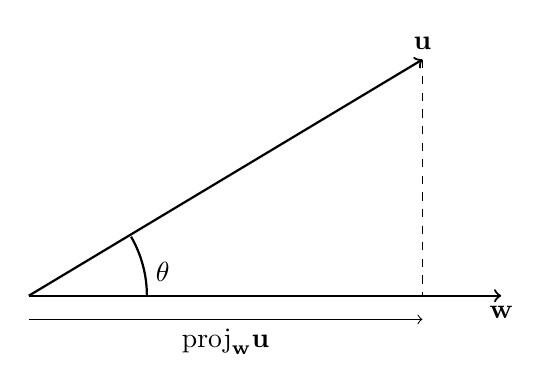
\begin{tikzpicture}
		% Draw vector w
		\draw[->, thick] (0,0) -- (6,0) node[anchor=north] {$\mathbf{w}$};

		% Draw vector u
		\draw[->, thick] (0,0) -- (5,3) node[anchor=south] {$\mathbf{u}$};

		% Projection line
		\draw[dashed] (5,3) -- (5,0) node[anchor=north] {};

		% Angle theta
		\draw[thick] (1.5,0) arc (0:30:1.5);
		\node at (1.7,0.3) {$\theta$};

		% Label projection of u on w
		\draw[->] (0,-0.3) -- (5,-0.3) node[midway,below] {$\text{proj}_{\mathbf{w}}\mathbf{u}$};
	\end{tikzpicture}
\end{center}
\[
	\text{scal}_{\mathbf{w}}\mathbf{u} = |\mathbf{u}| \cdot \cos\theta = \frac{\mathbf{w} \cdot \mathbf{u}}{|\mathbf{w}|}
\]
\[
	\text{proj}_{\mathbf{w}} \mathbf{u} = |\mathbf{u}| \cos \theta \left( \frac{\mathbf{w}}{|\mathbf{w}|} \right)
\]
\[
	\text{proj}_{\mathbf{w}} \mathbf{u} = \left( \frac{\mathbf{w} \cdot \mathbf{u}}{\mathbf{w} \cdot \mathbf{w}} \right) \mathbf{w}
\]
\[
	S(t) = \int_a^t \left| \vec{r}'(s) \right| \, ds.
\]
\[
	\frac{d}{dt} \vec{r}(S^{-1}(t)) = \frac{\vec{r}'(S^{-1}(t))}{\left| \vec{r}'(S^{-1}(t)) \right|}.
\]
\[
	\kappa(t) = \frac{|\vec{T}'(t)|}{|\vec{r}'(t)|}
\]
\[
	\kappa (t) = \frac{\lvert \vec{a} \times \vec{v} \rvert}{\lvert \vec{v} \rvert^3}, \quad \kappa (t) = \frac{1}{\lvert \vec{v} \rvert} \left\lvert \frac{d\vec{T}}{dt} \right\rvert, \quad \kappa (t) = \lvert \frac{d\vec{T}}{ds} \rvert
\]
\[
	|\vec{a}_\perp(t)| = \frac{|\vec{v}(t) \times \vec{a}(t)|}{|\vec{v}(t)|} = |\vec{v}(t)|^2 \cdot \kappa(t)
\]
\[
	|\vec{a}_\parallel(t)| = \frac{d}{dt}|\vec{v}(t)| = \frac{d^2}{dt^2} \int_0^t |\vec{v}(p)| dp = \frac{d^2}{dt^2} s(t)
\]
\[
	\vec{a}(t) = |\vec{a}_\perp(t)| \cdot \frac{\vec{T}'(t)}{|\vec{T	}'(t)|} + |\vec{a}_\parallel(t)| \cdot \frac{\vec{r}'(t)}{|\vec{r}'(t)|}
\]
\[
	\vec{B} = \vec{T} \times \vec{N} = \frac{\vec{v} \times \vec{a}}{|\vec{v} \times \vec{a}|}
\]
\[
	\vec{T} = \frac{\vec{r}'(t)}{|\vec{r}'(t)|}
\]
\[
	\vec{N} = \frac{\vec{T}'(t)}{|\vec{T}'(t)|}
\]
\[
	\frac{d\vec{B}}{dt} = -\tau \vec{N}
\]
\[
	\tau = \frac{\vec{B}'(t) \cdot \vec{N}(t)}{|\vec{r}'(t)|}
\]
\[
	\vec{B} = \frac{\vec{v} \times \vec{a}}{|\vec{v} \times \vec{a}|}
\]
\[
	\tau = \frac{(\vec{v} \times \vec{a}) \cdot \vec{a}'}{|\vec{v} \times \vec{a}|^2}
\]
\end{multicols}

\pagebreak

\[
		\text{det}(M) = \det\begin{pmatrix} a & b \\ c & d \end{pmatrix} = ad - bc
\]

\[
	H(x, y) = \begin{bmatrix}
		f_{xx}(x, y) & f_{xy}(x, y) \\
		f_{yx}(x, y) & f_{yy}(x, y)
	\end{bmatrix}
\]

\begin{center}
	\begin{enumerate}
		\item If \( \text{det}(H) > 0 \) and \( f_{xx}(a, b) > 0 \), then \( f(a, b) \) is a \emph{local minimum}.
		\item If \( \text{det}(H) > 0 \) and \( f_{xx}(a, b) < 0 \), then \( f(a, b) \) is a \emph{local maximum}.
		\item If \( \text{det}(H) < 0 \), then \( (a, b) \) is a \emph{saddle point}.
		\item If \( \text{det}(H) = 0 \), the test is \emph{inconclusive}.
	\end{enumerate}
\end{center}

\begin{center}
	\begin{tabular}{|c|c|}
		\hline
		\textbf{Curve/Surface} & \textbf{Equation}                                                     \\
		\hline
		\( y = f(x) \)         & \( y = f'(a)(x - a) + f(a) \)                                         \\
		\( z = f(x, y) \)      & \( z = c + \nabla f(a, b) \cdot \langle x - a, y - b \rangle \)       \\
		\( F(x, y, z) = D \)   & \( \nabla F(a, b, c) \cdot \langle x - a, y - b, z - c \rangle = 0 \) \\
		\hline
	\end{tabular}
\end{center}

\end{document}
